\documentclass[tcc, capa, capa-completa, english]{ufxc}

% capa: imprime a parte da frente da capa em uma única página
% capa-completa: imprime a versão completa da capa, com a parte da frente, verso, lombada e as orelhas

% =====================================================
% Pacotes usados no projeto
% =====================================================

\usepackage[style=abnt, noslsn]{biblatex} %, language=brazil
\usepackage{tocloft}
\let\printglossary\relax
\let\theglossary\relax
\let\endtheglossary\relax

% \usepackage[brazilian,hyperpageref]{backref}   % Paginas com as citações na bibl
% \usepackage[alf]{abntex2cite} % Citações padrão ABNT

\usepackage[noredefwarn, acronyms, symbols]{glossaries}
\usepackage[lined,boxed,ruled,commentsnumbered]{algorithm2e}


% \usepackage{pgf}
% \usepackage{tikz}
% \usepackage{hhline}
% \usepackage{xfrac}
% \usepackage[export]{adjustbox} % http://tex.stackexchange.com/questions/163246/resize-a-tabular-object-to-textwidth
% \usepackage{rotating}
% \usepackage{pdflscape}
% \usepackage{amsmath}
% \usepackage{amstext}
% \usepackage{amsfonts}
% \usepackage{amssymb}
% \usepackage{mathtools}
% \usepackage{amsthm}
% \let\openbox\relax
% \usepackage{bm}

% % \DeclarePairedDelimiter\floor{\lfloor}{\rfloor}
% \usepackage[makeroom]{cancel}
% \usepackage{color}    % Possibilita o uso de cores no documento
% \usepackage{colortbl}
\usepackage{subfig} % Usado para separar figuras em sub-figuras (ambiente subfloat) 
% \usepackage{scalefnt}
\usepackage{multirow}
% \usepackage{iflang} %there is a warning which will be corrected in future texmf dist.
% \usepackage[lined,boxed,ruled,commentsnumbered]{algorithm2e}
% \usepackage{soul}

% \usepackage{xspace} %In init/math

\usepackage{todonotes}
\usepackage{tabularx}
\usepackage{pgfgantt}

% Code Snippets
\usepackage{listings}
\renewcommand{\lstlistingname}{Código}
\lstset{
    basicstyle=\scriptsize\ttfamily,
	numbers=left,
	stepnumber=1,
	numbersep=-0.5em,
	keywordstyle=\color{blue},
	commentstyle=\color{black},
	stringstyle=\color{black},
    numberstyle=\scriptsize\ttfamily\color{black},
	frame=single,
	tabsize=2,
	float,
	language=C++,
	captionpos=t,
	showstringspaces=false,
	backgroundcolor=\color{white},
	morekeywords = {Array2D, __parallel__, Mask2D, Stencil2D},
	emph={
		pragma,
		omp,
		parallel,
		reduction,
		schedule,
		private,
		shared
	},
	emphstyle={\color{blue}}%
}

% =====================================================
% Local/data
% =====================================================

\local{Florianópolis}
\data{01}{Junho}{2019}

% =====================================================
% Informações do programa
% =====================================================

\instituicao{Universidade Federal de Santa Catarina}
\centro{Centro Tecnológico}
\departamento{Departamento de Informática e Estatística}
\grau{bacharel}
\curso{Ciência da Computação}
\coordenador{Nome do Coordenador do Curso}

% =====================================================
% Título e Informações sobre o autor
% =====================================================

\titulo{A Inter-Cluster Communication Module of a Hardware Abstraction Layer for Lightweight Manycore Processors}
% \subtitulo{}

\autor{João Vicente}{Souto}

%formato para orientador e coorientador:
%\orientador[genero]{titulação}{primeiros nomes}{sobrenome}{Universidade}
\orientador{Dr.}{Márcio Bastos}{Castro}{Universidade Federal de Santa Catarina}
\coorientador{Me.}{Pedro Henrique}{Penna}{Université Grenoble Alpes}

% =====================================================
% informações da banca
% =====================================================
% * assume-se que o orientador é parte da banca avaliadora
\coorientadorNaBanca{}

%formato para membro da banca
%\membroBanca{Nome}{Afiliação}
\membroBanca{Prof$^a$. Dr$^a$. Membro A. First}{Universidade Federal de Santa Catarina}
\membroBanca{Prof. Dr. Membro B.}{Universidade Federal de Santa Catarina}
\membroBanca[video]{Prof. Dr. Membro C.}{Universidade Federal de Santa Catarina}


% =====================================================
% Informações do trabalho
% =====================================================

%as palavras-chave devem ser definidas antes do início do documento pois
%a capa e também a lista catalográfica dependem delas...
% \palavrasChave{{latex},{abntex},{editoração de texto}}
%perceba a maneira como cada palavra chave é definida. Tal modo deve ser 
%mantido para a correta geração da ficha catalográfica

% por algum motivo ainda não identificado, ocorre um erro se os dois não forem definidos e as palavras não são impressas na ficha catalográfica
\palavrasChave{{Template}, {Ufsc}, {Latex}, {BU}}
\palavrasChave[english]{{Template}, {Ufsc}, {Latex}, {BU}}

% ---
% compila o indice
% ---
\makeindex
% ---

% {glossaries} package
% \makeglossaries
% \loadglsentries{init/acronyms}
% \loadglsentries{init/symbols}
\glsdisablehyper

%%%%%%%%%%%%%%%%%%%%%%%%%%%%%%%%%%%%%%%%%%%%%%%%%%%%%%%%%%%%%%%%%%%%
%%% Acronyms list                                                %%%
%%%%%%%%%%%%%%%%%%%%%%%%%%%%%%%%%%%%%%%%%%%%%%%%%%%%%%%%%%%%%%%%%%%%
%%% Importante:                                      
%%% - A lista PRECISA SER MANTIDA ORDENADA
%%%%%%%%%%%%%%%%%%%%%%%%%%%%%%%%%%%%%%%%%%%%%%%%%%%%%%%%%%%%%%%%%%%%

%A
\xnewacronym[amp]{AMP}{Asymmetric Multi-Processing}
\xnewacronym[anova]{ANOVA}{Analysis of Variance}
\xnewacronym[api]{API}{Application Programming Interface}

%B

%C
\xnewacronym[cnoc]{C-NoC}{Control Network-on-Chip}
\xnewacronym[cmp]{CMP}{Chip Multiprocessor}
\xnewacronym[cow]{COW}{Copy-On-Write}
\xnewacronym[cpu]{CPU}{Central Processing Unit}

%D
\xnewacronym[dnoc]{D-NoC}{Data Network-on-Chip}
\xnewacronym[dma][longplural={Direct Memory Accesses}]{DMA}{Direct Memory Access}
\xnewacronym[dram][longplural={Dynamic Random Access Memories}]{DRAM}{Dynamic Random Access Memory}
\xnewacronym[dtlb]{DTLB}{Data Translation Lookaside Buffer}

%E

%F
\xnewacronym[flops]{FLOPS}{Floating-point Operations per Second}
\xnewacronym[fos]{FOS}{Factored Operating System}
\xnewacronym[fpga]{FPGA}{Field Programmable Gate Array}

%G
\xnewacronym[gpu]{GPU}{Graphics Processing Unit}

%H
\xnewacronym[hal]{HAL}{Hardware Abstraction Layer}
\xnewacronym[hpc]{HPC}{High-Performance Computing}

%I
\xnewacronym[iid]{i.i.d}{Independent and Identically Distributed}
\xnewacronym[ipc]{IPC}{Inter-Process Communication}
\xnewacronym[isa]{ISA}{Distributed Hash Table}
\xnewacronym[itlb]{ITLB}{Instruction Translation Lookaside Buffer}
\xnewacronym[ieee]{IEEE}{Institute of Electrical and Electronics Engineers}

%J
\xnewacronym[jtlb]{JTLB}{Join Translation Lookaside Buffer}

%K

%L
\xnewacronym[lfour]{L4}{L4 Microkernel}
\xnewacronym[ltlb]{LTLB}{Locked Translation Lookaside Buffer}

%M
\xnewacronym[mimd]{MIMD}{Multiple Instruction Multiple Data}
\xnewacronym[misd]{MISD}{Multiple Instruction Single Data}
\xnewacronym[mmio]{MMIO}{Memory-Mapped I/O}
\xnewacronym[mmu]{MMU}{Memory Management Unit}
\xnewacronym[moosca]{MOOSCA}{Manycore Operating System for Safety-Critical Application}
\xnewacronym[mos]{mOS}{multi Operating System}
\xnewacronym[mpi]{MPI}{Message Passing Interface}
\xnewacronym[mpsoc]{MPSoC}{Multiprocessor System-on-Chip}
\xnewacronym[mpu]{MPU}{Memory Protection Unit}

%N
\xnewacronym[noc]{NoC}{Network-on-Chip}
\xnewacronym[norma]{NoRMA}{No Remote Memory Access}
\xnewacronym[nos]{nOS}{Nano-Sized Operating System}
\xnewacronym[numa]{NUMA}{Non-Uniform Memory Access}

%O
\xnewacronym[os]{OS}{Operating System}

%P
\xnewacronym[pe]{PE}{Processing Element}
\xnewacronym[pgas]{PGAS}{Partitioned Global Address Space}
\xnewacronym[pmca]{PMCA}{Programmable Manycore Accelerator}
\xnewacronym[pmio]{PMIO}{Port-Mapped I/O}
\xnewacronym[posix]{POSIX}{Portable Operating System Interface}
\xnewacronym[pucminas]{PUC Minas}{Pontifical Catholic University of Minas Gerais}

%Q
\xnewacronym[qos]{QoS}{Quality of Service}

%R
\xnewacronym[rab]{RAB}{Remapping Address Block}
\xnewacronym[ram][longplural={Random Access Memories}]{RAM}{Random Access Memory}
\xnewacronym[risc]{RISC}{Reduced Instruction Set Computer}
\xnewacronym[rm]{RM}{Resource Manager}
\xnewacronym[rma][longplural={Remote Memory Accesses}]{RMA}{Remote Memory Access}
\xnewacronym[rmem][longplural={Remote Memories}]{RMem}{Remote Memory}

%S
\xnewacronym[simd]{SIMD}{Single Instruction Multiple Data}
\xnewacronym[sisd]{SISD}{Single Instruction Single Data}
\xnewacronym[shm]{SHM}{POSIX Shared Memory}
\xnewacronym[smp]{SMP}{Symmetric Multi-Processing}
\xnewacronym[soc]{SoC}{System-on-a-Chip}
\xnewacronym[spm][longplural={Software-managed Scratchpad Memories}]{SPM}{Software-managed Scratchpad Memory}
\xnewacronym[sram][longplural={Static Random Access Memories}]{SRAM}{Static Random Access Memory}
	
%T
\xnewacronym[tlb]{TLB}{Translation Lookaside Buffer}

%U
\xnewacronym[ufsc]{UFSC}{Federal University of Santa Catarina}
\xnewacronym[uga]{UGA}{University of Grenoble Alpes}
\xnewacronym[uma][longplural={Uniform Memory Accesses}]{UMA}{Uniform Memory Access}

%V
\xnewacronym[vliw]{VLIW}{Very Long Instruction Word}

%W
\xnewacronym[watts]{W}{Watts}

%%% Local Variables:
%%% mode: latex
%%% TeX-master: "main"
%%% End:

%% List of Symbols

\newglossaryentry{jcost}%
{%
	name={\ensuremath{j_{\text{cost}}}},
	description={The lagrangian rate-distortion cost of selecting a given candidate as reference},
	sort={J},
	type=symbols
}

\newglossaryentry{jlambda}%
{%
	name={\ensuremath{\lambda}},
	description={The Lagrange multiplier.},
	sort={lambda},
	type=symbols
}

% numbers 

\newglossaryentry{naturalnumbers}%
{%
	name={\ensuremath{\mathbb{N}}},
	description={The set of natural numbers. },
	sort={Number Natural},
	type=symbols
}

\newglossaryentry{rationalnumbers}%
{%
	name={\ensuremath{\mathbb{Q}}},
	description={The set of rational numbers. },
	sort={Number Rational},
	type=symbols
}

\newglossaryentry{integernumbers}%
{%
	name={\ensuremath{\mathbb{Z}}},
	description={The set of integer numbers. },
	sort={Number Integer},
	type=symbols
}

\newglossaryentry{realnumbers}%
{%
	name={\ensuremath{\mathbb{R}}},
	description={The set of real numbers. },
	sort={Number Real},
	type=symbols
}


%\glsaddall
\usepackage{xspace}
\DeclareMathOperator*{\argmin}{arg\,min}

\newtheorem{theorem}{{Theorem}}
\newtheorem{property}{Property}

\newtheorem{definition}{Definition}
\newtheorem{lemma}{Lemma}[definition]

\DeclareMathAlphabet{\mathcal}{OMS}{cmsy}{m}{n}
\DeclareMathAlphabet{\mathbfcal}{OMS}{cmsy}{b}{n}




\newcommand\qedsymbol{$\blacksquare$} %renewcommand o

\makeatletter
\renewcommand*\env@matrix[1][*\c@MaxMatrixCols c]{%
  \hskip -\arraycolsep
  \let\@ifnextchar\new@ifnextchar
  \array{#1}}
\makeatother

\newcommand{\jcost}{\gls{jcost}\xspace}
\newcommand{\jlambda}{\gls{jlambda}\xspace}

\newcommand{\naturals}{\gls{naturalnumbers}}
\newcommand{\integers}{\gls{integernumbers}}
\newcommand{\reals}{\gls{realnumbers}}

\newcommand{\primes}{\ensuremath{\mathbb{P}}}
\newcommand{\rationals}{\ensuremath{\mathbb{Q}}}
\newcommand{\complex}{\ensuremath{\mathbb{C}}}
\newcommand{\quaternions}{\ensuremath{\mathbb{H}}}


\addbibresource{references.bib} % {biblatex} package
% \bibliography{references}

%%these will be used in the large cover
% \pequenoResumo{Esse é o pequeno resumo que vai aparecer na orelha orelha direita da capa.}
% \bairro{Trindade}
% \cidade{Florianópolis}
% \estado{SC}

% =====================================================
% Comandos do usuário
% =====================================================

\newcommand{\note}[1]{\textbf{\textcolor{blue}{\hl{#1}}}} % {color, soul} package

% adiciona automaticamente \centering em ambientes tipo float
\makeatletter
\g@addto@macro\@floatboxreset\centering
\makeatother

% Caso prefira referenciar acronimos com \ac e \acp.
% \newcommand{\ac}[1]{\gls{#1}}
% \newcommand{\acp}[1]{\glspl{#1}}

% =====================================================
% Início do documento
% =====================================================
\begin{document}

% Seleciona o idioma do documento (conforme pacotes do babel)
\selectlanguage{english}

% =====================================================
% Pré-textuais
% =====================================================

% \imprimircapa
\imprimirfolhaderosto* % (o * indica que haverá a ficha bibliográfica)

% \imprimirFichaCatalografica{} % pode passar pdf por parametro
% \input{pretextuais/errata}
% \inserirFolhaDeAprovacao{} % pode passar pdf por parametro

% \input{pretextuais/dedicatoria}
% \input{pretextuais/agradecimentos}
% % ---
% Epígrafe
% ---
\begin{epigrafe}
    \vspace*{\fill}
	\begin{flushright}
		\textit{``Uma epígrafe\\
		bem bonita.\\
		(Fulano de Tal)
		''}
	\end{flushright}
\end{epigrafe}
% ---
% % resumo em inglês
\begin{resumo}[brazil]
Resumo aqui.
\end{resumo}

\begin{resumo}[english]
% - Where do manycores from?
    For some years now, computer systems grew the core parallelism and improved diverse other architectural aspects to soften the impact of the frequency barrier achieved, looking for continuous scale performance.
    However, for supercomputers to reach processing power (FLOPS) in the \exascale (10$^{18}$), computer systems must take into account their energy consumption~\cite{darpa:exascale}. Therefore, a new architecture category of processors, denominated \textit{lightweight} \manycores, emerged to provide high parallelism with low-power consumption.

% - Manycores characteristics
    These new processors
    (i) integrate thousands of low-power cores in a single die; 
    (ii) are designed to cope with \mimd workloads;
    (iii) rely on a high-bandwidth \noc for fast and reliable message-passing communication;
    (iv) present constrained memory systems; and
    (v) frequently feature a heterogeneous configuration.
    Some industry-successful examples of lightweight manycores are
    the \mppa~\cite{DeDinechin2013-1};
    the \epiphany~\cite{Olofsson2014}; and
    the \taihulight~\cite{Zheng2015}.

% Motivation
% - Why is development on manycores difficult?
    Jointly with further performance scalability and energy efficiency, manycores brought a new set of challenges in software development coming from their architectural particularities.
    Precisely, these particularities force developers 
    (i) to adopt a message-passing programming model; 
    (ii) to deal explicitly with cache coherency;
    (iii) to take data tiling and prefetching approach for handling the small local memory and multiple address spaces; and
    (iv) to manage the complexity of development to commonly heterogeneous architecture.
% - Why develop for their processors?
    

% Challenges and Problem Definition
% - Why these problems exist? (Because the existing OSes does not handle architecture particularities)
% - These particularities prevent common OSes that easy portated without a complex redesign. And existing OSes does not account some architectural points.

% Goals and Contributions
% - Redesign from scratch around all their tight architectural constraints.
% - Focus on addressing first-order programmability challenges
% - Introducing generic and flexible HAL for lightweight manycores
\end{resumo}

% \inserirListaDeFiguras{}
% \inserirListaDeTabelas{}
% \inserirListaDeAcronimos{}
% \inserirListaDeSimbolos{}
% \inserirListaDeAlgoritmos{}

\inserirSumario{}

% =====================================================
% Corpo do trabalho
% =====================================================

\textual

\chapter{Introduction}
\label{ch.intro}

	% Context
	% Historical background
	% Frequency barrier
	For several years, the increase in the frequency of processors was
	employed as the main technique for achieving performance
	improvements. However, as a side effect, the temperature of
	processors started rising to high values, thus imposing a physical
	limit to the aforementioned technique. Alternatively, the constant
	improvement of semiconductor technology helped to mitigate the
	impact of this problem, allowing the industry to build more powerful
	processors with the same frequency. Therefore, knowing the
	frequency barrier and the imminent end of Moore's
	Law~\cite{moore:1965}, the academy and industry began to research
	and invest in alternatives to keep increasing the processing power
	of computer systems.

	% Improves architectural parts
	\autoref{fig:microprocessor-data} illustrates the paradigm shift
	that processors have gone through to the present day. From mid-2000,
	the frequency of processors tended to stagnate. The steady increase
	in transistors in the same chip area and the vast diversity of
	trade-offs to improve single-thread performance has softened the
	frequency impact on processors. Some significant trade-offs are
	different types of instruction sets, instruction parallelism,
	out-of-order processing techniques, branch prediction techniques,
	and various memory hierarchies. Then, in mid-2005, the performance
	of computer systems was pushed even further by increasing the number
	of processing cores in a single die. These architectures, called
	\textit{multicores}, allowed the continuous rise of the computing
	performance.

	The ever-increasing number of transistors and cores in a chip
	quickly led to the advent of \manycores. Notwithstanding, the line
	between \textit{multicores} and \manycores is very tenuous. Some
	researchers argue that the in latter architectures, losing a core it
	will not significantly impact the performance of the platform. A
	system is classified as \manycore when there is a need for
	distributed memory and on-chip networking~\cite{freitas:thesis}.

	\begin{figure}[t]
		\centering%
		\caption{Multiprocessor evolution.}%
		\label{fig:microprocessor-data}%
		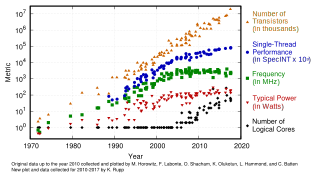
\includegraphics[width=.85\textwidth]{42-years-processor-trend.pdf}%
		\fonte{Adapted from \citeonline{url:microprocessor-trend-data}.}%
	\end{figure}

	% From multicore to manycores and Manycores characteristics
	Yet another classification for manycores is based on
	their ratio between processing speed, measured by the number of \flops, and power consumption,
	in \watts. \autoref{fig:microprocessor-data} pictures that even as the
	number of cores increasing, typical power has not grown uncontrollably.
	For instance, to achieve \exascale ($10^{18}$ \flops), the US Department
	of Defense issued a report stipulating the energy efficiency of a
	supercomputer should be around 50 GFLOPS/\watts~\cite{darpa:exascale}. 
	To cope with this energy constraint, a new class of
	parallel processors, called \lightweight \manycores, emerged to
	provide high parallelism with low power consumption.
	Lightweight manycores differ from traditional large-scale
	multicores and manycores in several points: 

	\begin{itemize}
		\item They integrate thousands of low-power cores in a single die organized in clusters;
		\item They are designed to cope with \mimd workloads;
		\item They rely on a high-bandwidth \noc for fast and reliable message-passing communication;
		\item They have constrained memory systems; and
		\item They frequently feature a heterogeneous configuration.
	\end{itemize}

	Some industry-successful examples of \lightweight \manycores are the
	\mppa~\cite{DeDinechin2013-1}; the \epiphany~\cite{olofsson2014};
	and the \taihulight~\cite{zheng2015}. Together with superior performance
	scalability and energy efficiency, lightweight manycores brought a new
	set of challenges in software development coming from their
	architectural particularities. More precisely, these 
	introduced the following difficulties:

	\begin{itemize}
		\item \textit{Hybrid programming model:} due to the parallel and
		distributed nature of the architecture, engineers are frequently
		required to adopt a message-passing programming model to deal
		with the presence of rich \nocs~\cite{kelly2013} that
		interconnects clusters and a shared-memory model inside the
		cluster;

		\item \textit{Missing hardware support for cache coherency:} to
		reduce power consumption, theses processors do not feature cache
		coherency, which in turn forces programmers to handle it
		explicitly in software level and frequently calls out for a
		redesign in their applications~\cite{francesquini2015};

		\item \textit{Constrained memory system:} the frequent presence
		of multiple physical address spaces and small local memories
		require data tiling and prefetching to be handled by the
		software~\cite{Castro2016};

		\item \textit{Heterogeneous configuration:} the different
		programmable components on \lightweight \manycores turns the
		actual deployment of applications in a complex
		task~\cite{barbalace2015}.
	\end{itemize}

	% Challenges and Problem Definition
	Part of these challenges derives from existing runtimes and \oss.
	On the one hand, runtimes do not hide the characteristics of hardware
	making software development more challenging and non-portable, \eg they
	neither allow direct access to non-local data, nor the manipulation of
	them in a transparent way. Thus, fundamental \os mechanisms, such
	as core multiplexing, core partitioning, and process and data
	migration, may not be addressed. On the other hand, the complicated
	portability and scalability of traditional \oss with a monolithic
	kernels, which were designed to homogeneous hardware, is leading to
	alternative \os designs~\cite{Baumann2009, kluge2014, nightingale2009, rhoden2011}.

	% Goals and Contributions
	We believe that \oss for the next-generation of \lightweight
	\manycores must be redesigned from scratch to cope with their tight
	architectural constraints. Based on this idea, a new fully-featured
	distributed \os based on a multikernel approach~\cite{Baumann2009}
	is under investigations~\cite{penna2017-1,penna2017-2,penna2019}.
	The \nanvix \multikernel features a generic and flexible \hal for
	\lightweight \manycores that addresses the key issues encountered in
	the development for these processors. On top of the \nanvix
	\textit{\hal}, a microkernel is being designed and implemented
	to provide the bare bones of the most important system abstractions.

\section{Goals}
\label{sec.goals}

	Based on the aforementioned motivations, the primary and specific
	goals of this work are detailed next.

\subsection{Main Goal}
\label{sec.goals.main}

	The main goal of this undergraduate dissertation is to propose an
	\textit{Inter-Cluster Communication Module} to the \nanvix
	\textit{\hal} and port it to the \mppa manycore
	processor~\cite{DeDinechin2013-1}. This module exposes the
	essential abstractions that allow overlying layers to create richer
	communication services. Using this module, we also
	propose \textit{Inter-Cluster Communication Services} to the \nanvix
	\microkernel. This work is part of the collaborative project between
	\ufsc, \pucminas, and \uga to develop an \os for \lightweight \manycore platforms.

\subsection{Specific Goals}
\label{sec.goals.specific}

	\begin{itemize}
		\item Definition and proposal of an \textit{Inter-Cluster Communication Interface} for lightweight manycores;

		\item Implementation of the proposed interface in the \nanvix \hal for the \mppa lightweight manycore processor;
        
		\item Integration of the \nanvix \hal interface with the \nanvix \microkernel;
		
		\item Performance evaluation of \nanvix \microkernel implementation using synthetic micro-benchmarks that reproduce the \textit{collective communication routines} of the \mpi programming model.
	\end{itemize}

\section{Organization Of The Work}
\label{sec.organization}
	
	The remainder of this work is organized as follows.
	\autoref{ch.fundamentation} details the background of this work.
	\autoref{ch.related-work} discusses the principal related work.
	\autoref{ch.development} presents the development of this work.
	\autoref{ch.experiments} describes the experiments accomplished and
	discusses the results. Finally, \autoref{ch.conclusions} outlines
	the main conclusions of this work.

\chapter{Theoretical Fundamentation} % Or Fundamentals?
\label{ch.fundamentation}

    In this chapter, I introduce the fundamentals concepts related to the present work.

\section{Operating Systems Concepts}
    This section may come sooner (here).

\section{Multiple Processor Systems}

    According to Tanenbaum, exists three models of modern multiple processor architectures.
    A shared-memory multiprocessor, a message-passing multicomputer, and a wide area distributed systems.
    The sections below address the two first models presenting significant hardware and software concepts for the present monograph.

    \subsection{Multiprocessors}
    Hardware overview.
    Von Neumann Model -> Main Systems Organization
    - Maybe speak UMA and NUMA.
    - Flynn's Organization.
        
    Software overview.
    - OS
    - Processor, thread (simiraly with Flynn Organization)


\subsection{Multicomputers}
    Hardware overview.
    Software overview.

    Important: Low-level Software and User-level Software primarily for communication.

\subsection{Manycores}
    Focus on manycores.

    Use the above concepts to build the narrative on manycores.

\subsubsection{MPPA-256}
    Focus on manycores.

\section{Multikernel OS Concept}
    In this section, I will write about the Multikernel OS concept using Nanvix has an example.

\section{Microkernel OS Concept}
    Focus on microkernel.

\section{Nanvix HAL}
    Focus on HAL.
\chapter{Related Works}
\label{ch.related-works}

The proposal of this work is related to several other research works
on lightweight \manycores.
First, some research papers describing state-of-the-art \manycores
processors will be cited. Further, research on different \oses
proposed for such processors will be highlighted.

\section{Lightweight Manycore Processors}

	In addition to \mppa, many papers exemplify the wide variety of architectural
	possibilities of lightweight \manycores.
	For instance, Olofsson \etal~\cite{olofsson2014} introduce \epiphany as a
	high-performance energy-efficient \manycore architecture suitable for
	real-time embedded systems.
	The architecture consists of nodes communicating through three 2D mesh \nocs
	with a distributed shared-memory model without coherence protocol.
	Each node has one \risc \cpu, multi-banked local memory, a \dma engine,
	an event monitor and a network interface.
	The network interface exposes the three \nocs, where one is used for reading
	request, and the other two are used for write transactions destined for on-chip
	and off-chip.

	% DFMC 2015
	% On the other hand, Zheng \etal~\cite{zheng2015} presents a heterogeneous \manycore processor
	% named \dfmc for high performance computing systems.
	% \dfmc integrates computing processing elements clusters, management processing elements and
	% memory controllers which heterogeneous processor cores. Using a unified execution model,
	% \dfmc able a share-memory with suporting to cache coherence by  ......... => Is this lightweight?

	On the other hand, for help and facilitate on the \manycore processor design,
	Wallentowitz \etal~\cite{Wallentowitz2013} presents the open-source framework
	\optimsoc which allows build \manycore \soc and simulate them on a computer or
	synthesize them on a \fpga.
	The processing elements are \openrisc~\footnote{https://opencores.org/openrisc}
	processor organized in tiles.
	The central architectural element is the LISNoC, a \textit{packet-switched \noc}
	that implements virtual channels to avoid message-dependent deadlocks.
	The LISNoC support various network topologies, depending only on the tiles organization.
	Precisely, a \textit{network adapter} handles the memory transfers between
	tile and the memory and provide hardware means to a message-passing communication
	model among tiles.

	Similarly, Kurth \etal~\cite{Kurth2017} introduce the \hero, which unites an \arm
	host processor with a fully modifiable \riscv \manycore implemented on a \fpga.
	The \pmca uses a multi-cluster design em relies on multi-banked, called \spms.
	The data caches had substituted to a multi-channel \dma engine that copy data
	between a shared L1 \spm and remote \smps or shared main memory.
	Besides, exists different designs for the shared instruction caches and
	top-level interconnection such as bus or \noc.

\section{Operating Systems for Lightweight Manycore Processors}

	Baumann \etal~\cite{Baumann2009} proposed a new \os architecture for scalable multicore
	systems, called Multikernel.
	In their vision, the future of the \oses is on embracing the networked nature
	of the machines based on distributed systems ideas.
	Assuming the cores are independent nodes of a network, they build the tradicional
	\os functionalities as fully-featured processes.
	This processes communicate via message-passing and does not share the internal
	structures of the \os.
	The paper showed how expensive it is to maintain a state of the \os through
	shared-memory instead of exchanging messages and the subsequent increase of
	the complexity of cache-coherence protocols.
	The multikernel implementation, named Barelfish, follow three design principles.
	First, \textit{Make all inter-core communication explicit} turns the system
	amenable to human or automated analysis because processes communicate only
	through well-defined interfaces.
	Second, \textit{Make \os structures hardware-neutral} makes the hardware-independent
	code easy to debug, optimize, and facilitates the deploy the \os for new
	processor types, avoiding rework.
	And lastly, \textit{View \os state as replicated instead of shared} improve system
	scalability.

	\todo{Maybe take off mOS}
	In Wisniewski~\cite{Wisniewski2014} \etal, the concept of scalability was pushed
	to the extreme, thinking on \hpc.
	The principal motivation is the creation of an \os that simultaneously supports
	programmability, through support \linux \api, and provides a lightweight kernel
	to performance, scalability, and reliability.
	The \os, named \mos, provide as much of the compute hardware resources as
	possible to the \hpc applications. On the other hand, the Linux kernel
	component acts as a service that provides Linux functionalities.
	
	In like manner, Kluge \etal~\cite{Kluge2014} developed the \moosca.
	With \moosca, they introduce abstractions that are easily composed, called Nodes,
	Channels and, Servers.
	Where Nodes represent execution resources, Channels represent communication
	resources, \ie \noc resources, and lastly, Servers are nodes that provide
	services to client Nodes.
	To meet safety-critical requirements, they partition \manycore and distribute
	replicas of Servers turning the whole system is predictable.
	However, in order to deal with interferences in shared resources, such as \noc,
	usage policies are introduced to make possible the prediction of system behavior.

	Finally, Nightingale \etal~\cite{nightingale2009} presents the Helios \os to
	simplify the process of writing, deploy, and optimize an application across
	heterogeneous cores.
	They use the microkernel model, naming \textit{satellite kernel}, to export
	a uniform and straightforward set of \os abstractions.
	The most important design decisions were to avoid unnecessary remote communication
	by thinking about the penalty they have in \numa domains.
	Request the minimum of hardware primitives so that architectures with many
	constraints can be ported.
	Moreover, request the minimum hardware resources to support architectures with little
	computational power or memory constraints.

\section{Discussion}

	This will be written after checking previous chapters.
 \chapter{Proposal}
\label{ch.proposal}

\todo[inline]{Adicionar introdução ao capítulo, sumarizando o que será apresentado aqui. Indicar que as duas principais contribuições serão no ``inter-cluster communication module'' (o qual será portado para o MPPA) e nos ``communication services'' (que é mais genérico e poderá ser usado para outras plataformas).}

\section{Inter-Cluster Communication Module}

\subsection{Sync}

\todo[inline]{Quais são as funções? Como pretendes implementá-las? Quais são os recursos (API ou hardware) do MPPA que serão explorados para implementar essa interface?}

\subsection{Mailbox}

\todo[inline]{Quais são as funções? Como pretendes implementá-las? Quais são os recursos (API ou hardware) do MPPA que serão explorados para implementar essa interface?}

\subsection{Portal}

\todo[inline]{Quais são as funções? Como pretendes implementá-las? Quais são os recursos (API ou hardware) do MPPA que serão explorados para implementar essa interface?}

\section{Communication Services}

\todo[inline]{Quais são os serviços? Como pretendes implementá-los? Quais são os recursos (API ou hardware) do MPPA que serão explorados para implementar esses serviços?}

% \chapter{Experiments}
\label{ch.experiments}

    In this Chapter, ...

    \section{Micro-benchmarks}

        \subsection*{Ping-Pong}

            In this benchmark, I will write about ...

        \subsection*{Broadcast}

            In this benchmark, I will write about ...

        \subsection*{Scather}

            In this benchmark, I will write about ...

        \subsection*{Gather}

            In this benchmark, I will write about ...

        \subsection*{All-Gather}

            In this benchmark, I will write about ...

    \section{Results}

        In this section, I will write about ...
\chapter{Schedule}
\label{ch.schedule}

This chapter presents the schedule for the next activities
planned for the development of the undergraduate dissertation.

\section{Activities}
\label{sec:gantt}

\begin{figure}[!h]
	\caption{Chart Gantt of the Schedule.}

	\begin{center}
		\begin{ganttchart}[
			x unit=0.6cm,
			y unit title=0.6cm,
			y unit chart=0.6cm,
			hgrid,
			vgrid={{dotted, dotted, dotted, dotted, dotted, dotted}},
			% title label font=\3scriptsize,
			title/.append style={fill=gray!30},
			title height=1,
			bar/.append style={fill=gray!30,rounded corners=2pt},
			bar label font=\scriptsize,
			group label font=\scriptsize,
		]{7}{12}

		\gantttitle{\textbf{Meses}}{6} \\
		\gantttitle{\textbf{2019}}{6} \\
		\gantttitlelist{7,8,9,10,11,12}{1} \\
		\ganttbar{1. Writing the Implementation and Experiments.}{7}{9} \\
		\ganttbar{2. In-depth Writing of the Proposal.}{9}{10} \\
		\ganttbar{3. Presentation of the Undergraduate Dissertation.}{11}{11} \\
		\ganttbar{4. Review and Final Submission of the Undergraduate Dissertation.}{12}{12} \\

		\end{ganttchart}
	\end{center}

	\label{chart.gantt}
\end{figure}

	Figure \ref{chart.gantt} shows the planned activities and their durations visually.
	Beginning in July 2019, the final submission is planned for December 2019.
	In detail, the activities are described below:

	\begin{itemize}
		\item \textit{Writing the Implementation and Experiments:}
			Currently, the inter-cluster communication module has the \sync abstraction
			completed and part of the \mailbox abstraction.
			Since the \portal abstraction uses the same low-level mechanisms of the others
			abstractions, its implementation will be facilitated.
			The communication services already have prototypes developed by the author
			for a symmetric \os.
			In this way, the prototypes will need to be modified to use the \hal and
			modified for a master-slave model.
			Finally, micro-benchmarks will be developed to perform an analysis of the
			performance of the implemented services.
		\item \textit{In-depth Writing of the Proposal:}
			During September and October, this activity will be committed to improving
			this draft and detailing the project decisions chose and implementations produced.
			We will also describe the experiments performed and discuss the results obtained.
		\item \textit{Presentation of the Undergraduate Dissertation:}
			November will be dedicated to the development and preparation of the presentation
			of the work and the results achieved.
			So finally, to present the dissertation to the evaluators.
		\item \textit{Review and Final Submission of the Undergraduate Dissertation:}
			Finally, December will be dedicated to the correction of the issues indicated
			by the evaluators and finalized with the final submission of the dissertation.
	\end{itemize}

 \chapter{Conclusions}
\label{ch.conclusions}

Iniciamente, este trabalho apresentou um contexto histórico
dos processadores multicores até os tempos atuais.
Ao demonstrar a relação entre o aumento de núcleos e o consumo
de energia, foi discutido como a academia e a industria
começaram a desenvolver alternativas para amenizar as
barreiras tecnológicas que surgiram.
Contudo, mesmo os novos processadores que surgiram
se destacarem por causa do seu desempenho e consumo energético,
eles pecam em programabilidade e portabilidade proveniente
das suas características arquiteturais, tais como, modelo de
programação híbrido, subsistemas de memória restritivos,
falta de coerência de cache e configurações heterogênicas.
Parte das dificuldades deriva da incompletudo dos sistemas operacionais
e runtimes existentes em lidar com as severas restrições arquitetônicas.

Neste trabalho será desenvolvido um módulo de comunicação entre cluster
projetado em torno dos principais pontos no desenvolvimento de um
sistema operacional.
Como base, foi discutido aspectos de hardware e softwares
de arquiteturas paralelas e distribuidas.
Foram apresentadas modelos distintos de abordagens de sistemas operacionais
que podem a vir utilizar o módulo de comunicação.
Deste modo, para fornecer o esqueleto básico para tais sistemas operacionais,
três abstrações de comunicação foram propostas para a HAL com a preocupação
de prover qualidade de serviço.
Entre elas estão a abstração sync para criar barreiras distibuidas.
A abstração mailbox fornece a troca de mensagens pequenas com controle 
de fluxo.
E por fim, a abstração portal possibilita a troca de quantidade arbitrárias
de dados entre dois clusters.

Outra contribuição deste trabalho apresentada foram os 
serviços de comunicação para um sistema operacional baseado na abordagem microkernel.
Esses serviços providenciam a multiplexação dos recursos expostos pela HAL
e a verificação dos parâmetros necessários para cada abstração.
De forma geral, esses serviços exportam uma forma segura ao usuário
se beneficiando da não concorrência das estruturas internas do SO 
por causa da separação de responsabilidades de mestre e escravo.
Por fim, a proposta detalhou, de forma geral, vários aspectos
das implementações.
Devido ao fato dos serviços dependerem do módulo de comunicação da HAL
para serem desenvolvido, os tópicos associados ao módulo acabaram sendo
mais detalhados e melhor explorados.
Entretanto, a próxima versão da dissertação especificará com maior clareza
e objetividade ambas as contribuições deste trabalho.

% \chapter{Basic Concepts}
\label{ch.basic}

\section{Figure Examples}

Figure.

\begin{figure}[htb]
    \includegraphics[width=.4\textwidth]{images/ufsc_pb.pdf}
    
    \caption[Short Caption]{
        Long version of caption.
    }
\label{fig.cu}
\end{figure}

\subsection{Sub Figures}
Ref global Figure~\ref{fig.logo} and its subfigures~\ref{sfig.logoA}, \ref{sfig.logoB} and \ref{sfig.logoC}.

\begin{figure}[th]
    \subfloat[]{ \includegraphics[width=.2\linewidth]{images/ufsc_pb.pdf} \label{sfig.logoA} }
    \subfloat[]{ \includegraphics[width=.2\linewidth]{images/ufsc_pb.pdf} \label{sfig.logoB} }
    
    \subfloat[]{ \includegraphics[width=.2\linewidth]{images/ufsc_pb.pdf} \label{sfig.logoC} }
    
    \caption[Short Caption 2]{
        Long version of caption 2.
    }
\label{fig.logo}
\end{figure}

\section{Citations}
\citeonline{Wiegand03} made a nice job.
Citation \cite{Wiegand03}.

\section{Acronym}
See more in wiki\footnote{https://en.wikibooks.org/wiki/LaTeX/Glossary}.
\begin{enumerate}
    \item \gls{dag}.
    \item \glspl{dag}.
    \item \glspl{sram}.
    \item \gls{sram}.
    \item \acrfull{dag}
    \item \acrfullpl{dag}
    \item \test
    \item \test
    \item \tests
\end{enumerate}

\section{Table}

\begin{table}[h]
    \caption[Short Caption.]{
        Table caption here.
    }

    \resizebox{\linewidth}{!}{
        \begin{tabular}{@{}|c|c|c|c|c|c|c|c|c|c|@{}}
            \hline
              & \textbf{June}      & \textbf{July}      & \textbf{August}       & \textbf{September}     & \textbf{October}         & \textbf{November}         & \textbf{December}          & \textbf{January}         & \textbf{February}         \\ \hline
            \textbf{P1} & X & X  &   &   &   &   &   &   &   \\ \hline
            \textbf{P2} &   & X & X &   &   &   &   &   &   \\ \hline
            \textbf{P3} &   &  &  & X &   &   &   &   &   \\ \hline
            \textbf{P4} &   &  &  & X & X  & X  &   &   &   \\ \hline
            \textbf{P5} &   &   &   &   & X & X & X  &   &   \\ \hline
            \textbf{P6} &  &  &  &  &  &  & X & X  &   \\ \hline
            \textbf{P7} &   &   &   &   &   &   &   & X & X \\ \hline
            \textbf{P8} &   &   &   &   &   &   &   &   & X \\ \hline
        \end{tabular}
    }

\label{tab.table}
\end{table}

\section{Equations}
You can use symbols (\primes) from /init/math.

\begin{equation}
    % \displaystyle 
    \jcost(A, B) = + \jlambda \times A \in \integers \in \primes
\label{eq.test}
\end{equation}


\section{Algorithm}

\begin{algorithm}
    \DontPrintSemicolon % Some LaTeX compilers require you to use \dontprintsemicolon instead
    \KwIn{$A=[a_1, a_2, \ldots, a_n]$}
    \KwOut{Max value}
    $max \gets a_1$\;
    \For{$i \gets 2$ \textbf{to} $n$} {
      \If{$a_i > max$} {
        $max \gets a_i$\;
      }
    }
    \Return{$max$}\;
    
    \caption[Short]{
        Max finds the maximum number
    }
    \label{alg.max}
\end{algorithm}

\begin{algorithm}
    \DontPrintSemicolon % Some LaTeX compilers require you to use \dontprintsemicolon instead
    \KwIn{$A=[a_1, a_2, \ldots, a_n]$}
    \KwOut{Max value}
    $max \gets a_1$\;
    \For{$i \gets 2$ \textbf{to} $n$} {
      \If{$a_i > max$} {
        $max \gets a_i$\;
      }
    }
    \Return{$max$}\;
    
    \caption[Short]{
        Max finds the maximum number
    }
    \label{alg.max2}
\end{algorithm}

% =====================================================
% Pós-textuais
% =====================================================
\postextual
\printbibliography

% TODO
%\glossary

% \begin{apendicesenv}

% Imprime uma página indicando o início dos apêndices
\partapendices % this is something of abntex 
% https://github.com/abntex/abntex2/issues/133

\chapter{Quisque libero justo}

Mussum Ipsum, cacilds vidis litro abertis. 
Posuere libero varius. 
Nullam a nisl ut ante blandit hendrerit. Aenean sit amet nisi. 
Interagi no mé, cursus quis, vehicula ac nisi. 
Interessantiss quisso pudia ce receita de bolis, mais bolis eu num gostis. 
Aenean aliquam molestie leo, vitae iaculis nisl. 

\end{apendicesenv}

% \begin{anexosenv}

% Imprime uma página indicando o início dos anexos
\partanexos

\chapter{Morbi ultrices rutrum lorem}

    Mussum Ipsum, cacilds vidis litro abertis. 
    Posuere libero varius. Nullam a nisl ut ante blandit hendrerit. 
    Aenean sit amet nisi. Interagi no mé, cursus quis, vehicula ac nisi. 
    Interessantiss quisso pudia ce receita de bolis, mais bolis eu num gostis. 
    Aenean aliquam molestie leo, vitae iaculis nisl. 
    
\end{anexosenv}


%-----------------
% INDICE REMISSIVO
\phantompart
%\printindex
%-----------------

\end{document}
